\documentclass{book}
\pagestyle{headings}

\usepackage[latin1]{inputenc}   % codage du fichier source
\usepackage[T1]{fontenc}      % codage des fontes TeX
\usepackage[french]{babel}  % document en fran�ais
\usepackage{ifpdf}
\usepackage{pdfpages} % int�gre mes pdf dans les annexes 
\usepackage{lmodern} % Pour changer le pack de police
\usepackage{makeidx}
\usepackage{glossaries}

\makeglossaries
\makeindex
\title{Super titre}
\author{\textsc{Manet} St�phane}

\ifpdf
\pdfinfo{
  /Author (St�phane Manet)
  /Title (Super titre � placer ici)
  /Subject (Analyse du travail et didactique professionnelle � la RATP)
  /Keywords (LaTeX ATDC CNAM)}
\usepackage[pdftex,hyperindex,colorlinks=true]{hyperref}
\else
\usepackage[hypertex=true,hyperindex=true,colorlinks=false]{hyperref}
\fi

%\includeonly{intro-II,  outillage,cosmetique,jouets}
%\includeonly{pdf,memento,symboles,production}
%
%\includeonly{jouets,pdf}


\begin{document}

\maketitle %page de garde
	
\tableofcontents %sommaire
	
\frontmatter %on attaque l'intro

\chapter{introduction}
	\section{A propos du fond}
Ce rapport pr�sente mon activit� au sein de la RATP dans le cadre d'un terrain d'analyse qu'il m'a �t� demand� par les formateurs du CNAM, afin de valider le titre RNCP Responsable de projet de formation.\cite{col:McA}

Il compile donc trois �valuations : 

\begin{itemize}
	\item FAD111 : Analyse du travail, St�phane Balas
	\item FAD114 : Formation en situation de travail, Anne-Lyse Ulmann
	\item FAD115 : Acteurs machins, Jean-Louis Pontet
\end{itemize}

Ces trois �valuations portent sur diff�rents domaines d'exercice que l'on peut trouver dans le champs de la formation, au-del� de la p�dagogie m�me. L'analyse du travail et la didactique professionnelle, la mise en place d'une action de formation, et enfin l'analyse de donn�es statistiques, et des enjeux institutionnels. 

Le fait de travailler avec la RATP dans un contexte de Grand Paris est particuli�rement int�ressant.  

	\section{A propos de la m�thode}
Mon choix de regrouper ces �valuations sur le m�me terrain est avant tout un choix pratique. En effet, j'ai voulu rationaliser au mieux le temps qu'il m'�tait imparti pour r�aliser cette �tude et m'assurer que je puisse donner un maximum de temps � une seule analyse - de qualit� j'esp�re - plut�t que de multiplier les terrains au fur et � mesures des �valuations attendues. 

Il est � noter que j'ai r�alis� douze de ces �valuations sur deux ans, et que j'ai �galement du r�aliser des �tudes de terrain dans le cadre des FAD110 et FAD117 notamment, ainsi que des analyses de donn�es telles qu'une FAD103.

	\section{A propos de la forme}
Enfin, mon choix d'utiliser \LaTeX{} pour sa r�daction est un choix pratique et cognitif. Il me facilite la construction de mon document, et donc de ma pens�e. 

Pour des raison plus pratiques, c'est un entra�nement pour mon m�moire de l'ann�e prochaine, ma th�se etc. Il me permet �galement une gestion de la bibliographie plus structur�e.\footnote{Le syst�me \LaTeX{} est particuli�rement puissant pour g�rer les bibliographies.
	
J'ai cr�� 3 fichiers .bib distincts correspondant aux trois �valuations, afin de permettre � mes �valuateurs de recevoir une version ind�pendante correspondant � ses attentes. Toutefois, \LaTeX en g�n�re une bibliographie unique, tri�e par alphab�tiquement par auteurs, sans faire de doublons si un livre est cit� dans deux fichiers .bib diff�rents.}. % il conviendra sans doute d'expliciter tout cela en annexe et de faire un renvoi vers l'annexe ici. 

	\section{� propos de l'usage}
Le pr�sent document est sous licence Creative Commons BY-NC-SA 3.0.

Le code source du document, lui, est sous licence Apache 2.0.

Le code source est t�l�chargeable sur github.com : https://stephmnt.github.io/at-ratp.	

\mainmatter

\chapter{Analyse du travail et ing�nierie de la formation professionnelle}
\section{Des d�buts comme un diesel}
\subsection{mais pourquoi j'ai pas de titres :(}
La probl�matique � laquelle je me suis tout d'abord confront� est de savoir et comprendre qu'elle est ma place dans l'intervention d'une entreprise, telle que la RATP, et mieux discerner mes objectifs � cette occasion.

Lorsque j'ai commenc� � prospecter des terrains pour la FAD111	, j'ai \cite{col:ihrc}

\chapter{D�veloppement des comp�tences en situation de travail}
\part{Politique de formation et territoires}

\appendix

\chapter{proposition d'observation de terrain}
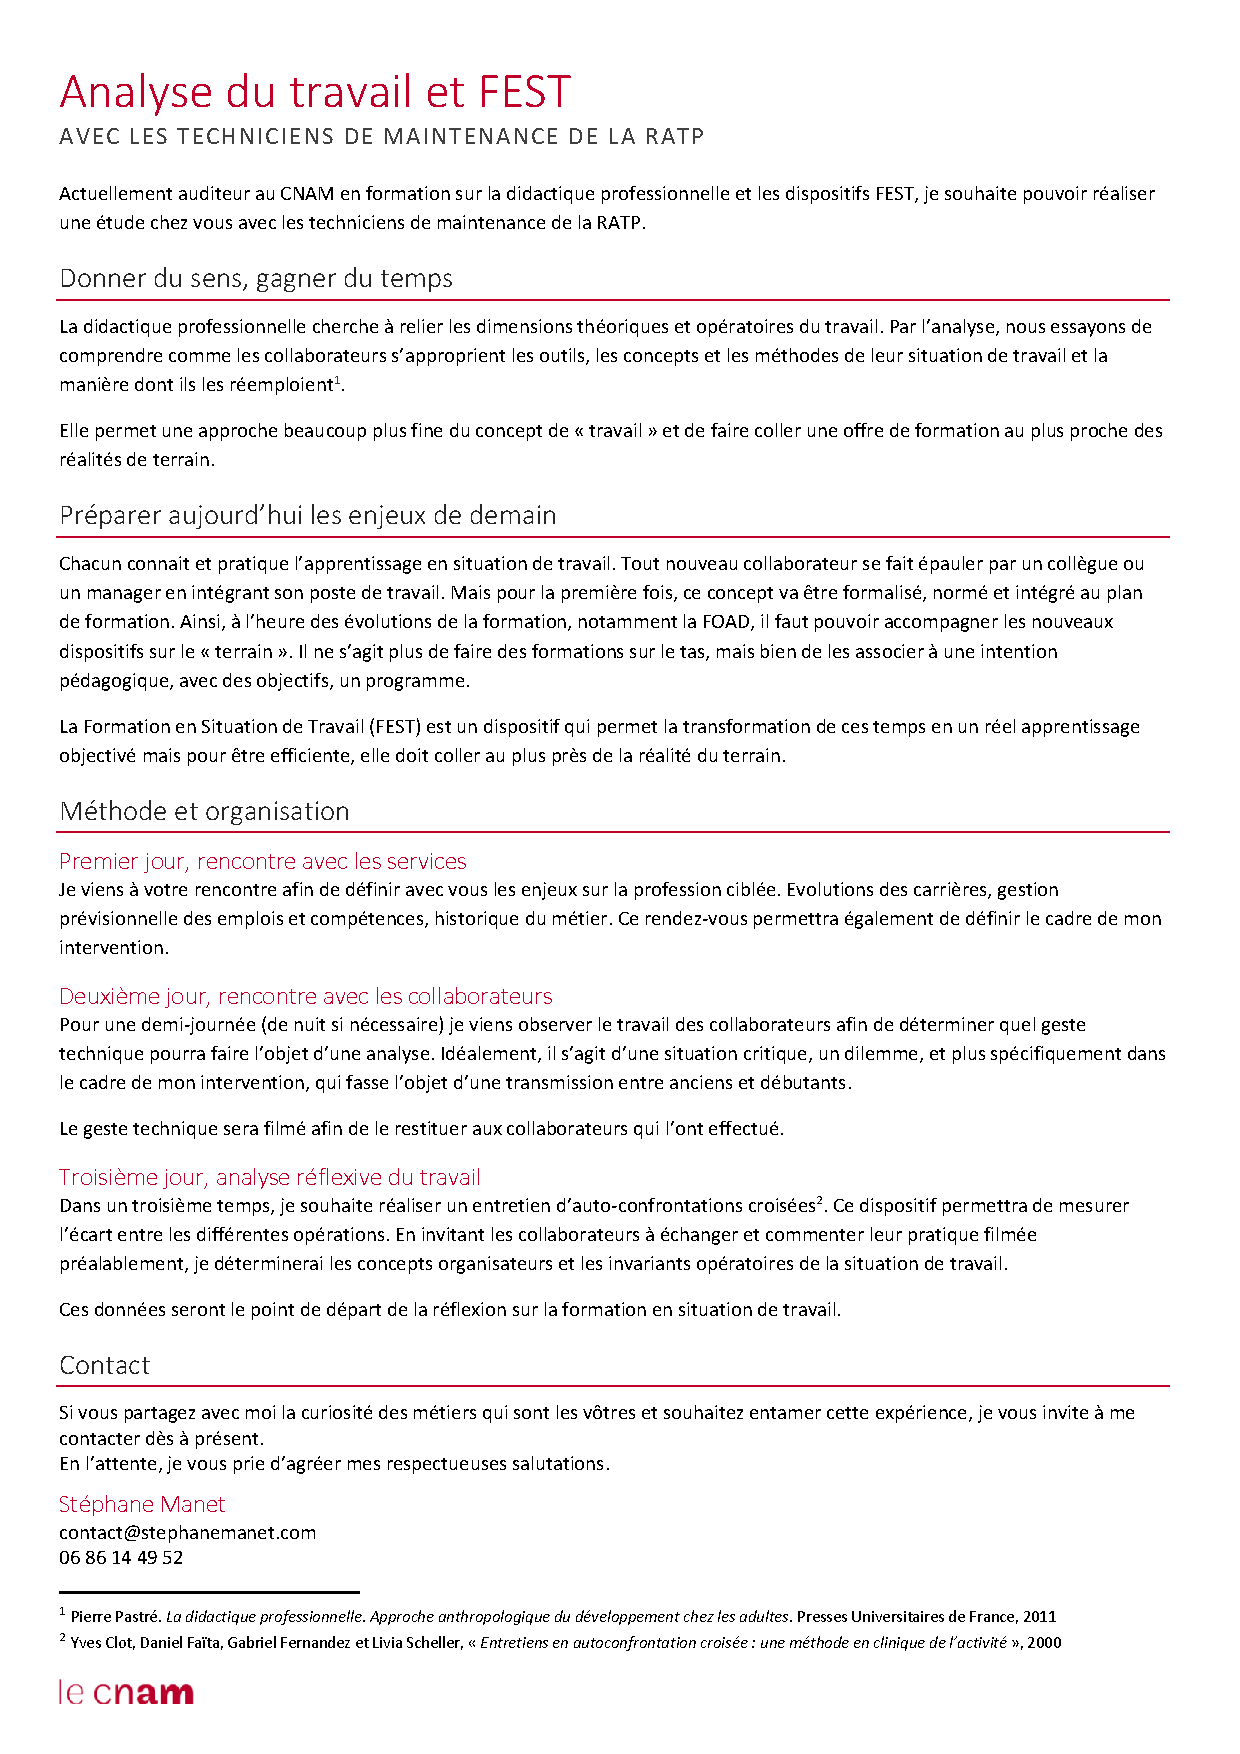
\includepdf[pages=-]{annexes/propa.pdf}
\chapter{Glossaire}
\printglossaries
\chapter{N'importe quoi d'autre}
\bibliographystyle{plain}
\bibliography{fad111.bib,fad114.bib,fad115.bib}



\backmatter

Epilogue


\end{document}